% !TEX root =  ../main.tex 

\section{Simulation study}
\label{sec: simulation_study}
The application of personalized schedules for patients from PRIAS program demonstrated that personalized schedules adapt according to the PSA and repeat biopsy history of each patient. However, the patients in PRIAS have already had their biopsies as per the PRIAS schedule, and hence evaluation of the efficacy of personalized schedules against the PRIAS schedule was not possible. To this end, we have performed a simulation study to compare 3 broad categories of schedules: Personalized schedules, PRIAS schedule and annual schedule. To compare the schedules we employ them for simulated patients enrolled in a hypothetical AS program, with the same entrance criteria as PRIAS. For these patients we simulate the evolution of PSA and the time of GR. Since our interest is only in the schedule of biopsies, we keep a fixed schedule for measurement of PSA levels. The hypothetical repeat biopsies are conducted until the GR is detected. Although Gleason scores are susceptible to inter-observer variation \citep{Gleason_interobs_var}, we assume that any biopsy conducted after the true GR time of a patient will lead to GR detection with 100\% certainty. We next present the details of the simulation study and the biopsy schedule evaluation criteria.

\subsection{Simulation setup}
\label{subsec : simulation_setup}
\subsubsection{Patient population}
For the simulation study we first select a population $\mathcal{P}$ of patients enrolled in AS. We assume that the PSA and hazard of GR for the patients from this population follows a joint model of the form postulated in Section \ref{subsec : jm_fit_prias}, with parameters $\boldsymbol{\theta}^{\mathcal{P}}$. These parameters are selected to be equal to the posterior mean of parameters $E[\boldsymbol{\theta} \mid \mathcal{D}^{PRIAS}]$ estimated from the joint model fitted to PRIAS dataset (Section \ref{subsec : param_estimates_jm_fit_prias}). To demonstrate the efficacy of personalized schedules for patients with early as well late failure times, we generated the patients in population $\mathcal{P}$ from 3 equal sized subgroups $G_1, G_2, G_3$. The baseline hazard for each of the three subgroups was assumed to be the hazard function of a Weibull distribution. The shape and scale parameters $(k, \lambda$) for this Weibull distribution are $(1.5, 4)$, $(3, 5)$ and $(4.5, 6)$ for $G_1, G_2$ and $G_3$ respectively. The effect of these parameters is that the variance in GR times is highest for $G_1$ and lowest for $G_3$, while the average GR is lowest in $G_1$ and highest in $G_3$.

\subsubsection{Generating PSA values and GR times}
From the population $\mathcal{P}$ we randomly sample a total of 408 datasets with 1000 patients each. For each of the simulated patients the PSA measurement schedule is same as that of PRIAS, i.e. every 3 months for first 2 years and every 6 months thereafter. Each simulated dataset is split into a training (750 patients) and a test (250 patients) part. Keeping in line with the notation for joint model in Section \ref{subsec : jm_specification}, the observed data in the $k$-th training dataset can be represented as $\mathcal{D}^k = \{l_{ki}, r_{ki}, \boldsymbol{y}_{ki}; i = 1, \ldots, 750\}$, where $\boldsymbol{y}_{ki}$ denotes the PSA levels for the $i$-th patient in the $k$-th training dataset. For a patient in the training dataset we generate a true event time $T^*_{ki}$ as well as a random and non-informative censoring time $C_{ki}$. When $T_{ki} < C^*_{ki}$, i.e. when the event is observed, then $l_{ki} = r_{ki} = T^*_{ki}$. When $C_{ki} < T^*_{ki}$, then $l_{ki} = C_{ki}$ and $r_{ki} = \infty$. For the patients in the test datasets censoring time is not generated. 

\subsubsection{Personalized schedules for test patients}
\label{subsubsec : sim_study_pers_sched_details}
We create personalized biopsy schedules only for the patients in the test dataset. To this end we first fit a joint model with the same specification as for PRIAS. to the training dataset. To model the baseline hazard we use a P-splines approach (Section \ref{subsec : jm_specification}). From the fitted joint model we obtain posterior distribution of parameters $p(\boldsymbol{\theta} \mid \mathcal{D}^k)$, which is required for the posterior predictive distribution $g(T^*_{kj})$ of the $j$-th test patient from the $k$-th dataset. While the posterior predictive distribution is sufficient for scheduling biopsies based on expected time of GR, the choice of time window $\Delta t$ (Section \ref{subsubsec : dynamic_risk_definitions}) has to be made for scheduling biopsies on the basis of dynamic risk of GR. In PRIAS and in most AS programs biopsies are done at a gap of 1 to 3 years. A gap of 1 year between biopsies detects GR the earliest, and in worst case the detection of GR can be delayed by 1 year. Being a clinically relevant period of time to differentiate between patients who obtain GR and those who don't, we choose a $\Delta t$ of 1 year. Further, in schedules based on dynamic risk of GR, for a test patient $j$, we choose a value of $\kappa$ which maximizes a binary classification measure (Section \ref{subsubsec : kappa_estimation}) at the last known repeat biopsy time $t$ of the patient. To this end the binary classification measures are first computed over a fine grid of $\kappa$ values in the interval $[0,1]$ using the training dataset and then the most optimal $\kappa$ is chosen.\\

To create personalized schedules we employ the algorithm described in Section \ref{subsec : pers_sched_algorithm}. The algorithm is run for 7 different settings, one each corresponding to the following: PRIAS schedule, annual schedule, expected time of GR, median time of GR, dynamic risk of GR with $\kappa$ chosen such that a) Youden's $J$ is maximized, b) $\text{F}_1$-Score is maximized. In addition to these a mixed approach (Section \ref{subsubsec : mixed_approach}) is also employed where a choice between median time of GR and dynamic risk of GR (Youden's $J$ maximized) is made before scheduling a biopsy.

\subsubsection{Estimation}
For the loss function in (\ref{eq : loss_func_sim_study}), we estimate $E[N^{bS}]$, $\mbox{var}[N^{bS}]$, $E[O^S]$ and $\mbox{var}[O^S]$ using pooled estimates of each from the 254 repetitions of the simulation study. The estimates are calculated separately for each of the 7 methods mentioned in Section \ref{subsubsec : sim_study_pers_sched_details}. The pooled estimates for a scheduling method $S$ are calculated as following:
\begin{align*}
\widehat{E[O^S]} &= \frac{\sum_{k=1}^{254} n_k \widehat{E[O^S_k]}}{\sum_{k=1}^{254} n_k}, \\
\widehat{\mbox{var}[O^S]} &= \frac{\sum_{k=1}^{254} (n_k - 1) \widehat{\mbox{var}[O^S_k]}}{\sum_{k=1}^{254} (n_k-1)}, 
\end{align*}
where $n_k$ are the number of test patients in the $k$-th simulation, $\widehat{E[O^S_k]} = \frac{\sum_{j=1}^{n_k}O^S_{kj}}{n_k}$ and $\widehat{\mbox{var}[O^S_k]} = \frac{\sum_{j=1}^{n_k}\big\{O^S_{kj} - \widehat{E[O^S_k]}\big\}^2}{n_k-1}$ are the estimated mean offset and estimated variance of the offset for the $k$-th simulation, respectively. The estimates for number of biopsies $N^{bS}$ are calculated similarly.


\subsection{Results}
From the simulations we calculated the pooled estimates of the mean and variance of number of biopsies/offset for the entire sample. The estimates are plotted in Figure \ref{fig : meanNbVsOffset} and also summarized in Table \ref{table : sim_study_pooled_estimates}. From the figure it is evident that those schedules which conduct less biopsies on average, have a higher average offset, and vice versa. For example, the annual schedule conducts 5.2 biopsies on average, which is the highest among all schedules, however it has the least average offset of 6 months as well. On the other hand the schedule based on expected time of GR conducts only 1.9 biopsies on average, the least among all schedules but it also has the highest average offset of 15 months. The schedule based on median time of GR performs almost the same as that based on expected time of GR. As mentioned earlier the variance in number of biopsies and offset are important as well. In this regard annual schedule has the largest $\mbox{var}[N^{bS}]$ since it attempts to contain the offset within an year, and consequently it has the least $\mbox{var}[O^S]$. Schedules based on expected and median time of GR perform the opposite in terms of variance.

\begin{figure}[!htb]
	\centering
    \captionsetup{justification=centering}
	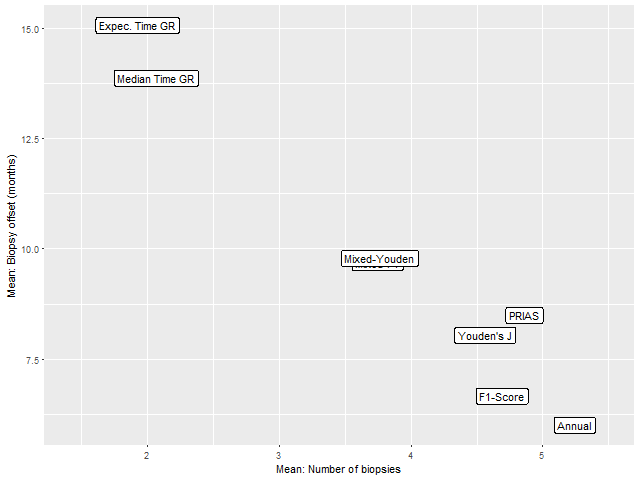
\includegraphics[width=0.8\textwidth]{images/sim_study/meanNbVsOffset_all.png}
	\caption{Estimated mean number of biopsies and mean offset (months) for the 7 scheduling methods using all patients. Method names are abbreviated for ease of graphing.}
	\label{fig : meanNbVsOffset}
\end{figure}

\begin{table}[!htb]
\centering
\captionsetup{justification=centering}
\caption{Pooled estimates of mean and variance of number of biopsies and offset for all patients.}
\label{table : sim_study_pooled_estimates}
\begin{tabular}{@{}lrrrrr@{}}
\toprule
Schedule           & Total Patients & $E[N^{bS}]$ & $E[O^{S}]$ & $\mbox{var}[N^{bS}]$ & $\mbox{var}[O^S]$ \\ \midrule
Annual              & 63386                  & 5.237           & 6.001               & 6.421          & 11.874             \\
PRIAS              & 63386                  & 4.858           & 8.464               & 5.523          & 74.223             \\
Expected time of GR & 63386                  & 1.923           & 15.066              & 1.422          & 146.319            \\
Median time of GR  & 63386                  & 2.066           & 13.899              & 2.003          & 139.773            \\
$\text{F}_1$-Score           & 63386                  & 4.683           & 6.654               & 4.807          & 18.834             \\
Youden's $J$             & 63386                  & 4.560            & 8.030                & 4.006          & 118.908            \\
Mixed approach     & 63386                  & 3.763           & 9.744               & 2.878          & 58.356             \\ \bottomrule
\end{tabular}
\end{table}

We observe that the PRIAS schedule performs more or less the same as annual schedule. Despite this the latter may be preferred over PRIAS since it conducts only 0.38 biopsies more on average, however unlike PRIAS it has very low variance of offset, thus guaranteeing early detection for everyone. If we compare the PRIAS schedule with dynamic risk of GR based schedules, we can see that the schedule where $\kappa$ is chosen after maximizing $\text{F}_1$-Score, performs better than in PRIAS schedule in all aspects. The schedule where $\kappa$ is chosen after maximizing Youden's $J$ has a very large $\mbox{var}[O^S]$ and hence is not preferable over PRIAS. The mixed approach combines the benefits of methods with low $E[N^{bS}]$ and $\mbox{var}[N^{bS}]$, and those methods with low $E[O^{S}]$ and $\mbox{var}[O^S]$. It conducts 1.5 less biopsies than annual schedule on average and at 9.7 months the mean offset is less than an year.\\

\begin{table}[!htb]
\centering
\captionsetup{justification=centering}
\caption{Pooled estimates of mean and variance of number of biopsies and offset for subgroup $G_1$.}
\label{table : sim_study_pooled_estimates_G1}
\begin{tabular}{@{}lrrrrr@{}}
\toprule
Schedule           & Total Patients & $E[N^{bS}]$ & $E[O^{S}]$ & $\mbox{var}[N^{bS}]$ & $\mbox{var}[O^S]$ \\ \midrule
Annual              & 21004                  & 4.306           & 6.024               & 9.788          & 11.747             \\
PRIAS              & 21004                  & 4.032           & 7.951               & 8.221          & 63.528             \\
Expected time of GR & 21001                  & 1.922           & 15.114              & 1.441          & 149.167            \\
Median time of GR  & 20937                  & 2.068           & 13.87               & 1.999          & 138.396            \\
$\text{F}_1$-Score           & 21061                  & 4.689           & 6.648               & 4.863          & 18.745             \\
Youden's $J$             & 21017                  & 4.581           & 8.045               & 3.979          & 121.309            \\
Mixed approach     & 21004                  & 3.252           & 10.361              & 4.611          & 73.781             \\ \bottomrule
\end{tabular}
\end{table}

\begin{table}[!htb]
\centering
\captionsetup{justification=centering}
\caption{Pooled estimates of mean and variance of number of biopsies and offset for subgroup $G_2$.}
\label{table : sim_study_pooled_estimates_G2}
\begin{tabular}{@{}lrrrrr@{}}
\toprule
Schedule           & Total Patients & $E[N^{bS}]$ & $E[O^{S}]$ & $\mbox{var}[N^{bS}]$ & $\mbox{var}[O^S]$ \\ \midrule
Annual              & 21160                  & 5.181           & 5.95                & 4.567          & 12.03              \\
PRIAS              & 21160                  & 4.817           & 8.569               & 3.98           & 75.716             \\
Expected time of GR & 21151                  & 1.927           & 15.078              & 1.447          & 144.333            \\
Median time of GR  & 21189                  & 2.062           & 13.947              & 1.994          & 140.633            \\
$\text{F}_1$-Score           & 21133                  & 4.666           & 6.663               & 4.726          & 18.956             \\
Youden's $J$             & 21167                  & 4.557           & 8.024               & 3.98           & 122.84            \\
Mixed approach     & 21160                  & 3.702           & 10.359              & 1.869          & 60.415             \\ \bottomrule
\end{tabular}
\end{table}

\begin{table}[!htb]
\centering
\captionsetup{justification=centering}
\caption{Pooled estimates of mean and variance of number of biopsies and offset for subgroup $G_3$.}
\label{table : sim_study_pooled_estimates_G3}
\begin{tabular}{@{}lrrrrr@{}}
\toprule
Schedule           & Total Patients & $E[N^{bS}]$ & $E[O^{S}]$ & $\mbox{var}[N^{bS}]$ & $\mbox{var}[O^S]$ \\ \midrule
Annual              & 21222                  & 6.214           & 6.03                & 3.118          & 11.851             \\
PRIAS              & 21222                  & 5.717           & 8.866               & 2.977          & 82.915             \\
Expected time of GR  & 21234                  & 1.921           & 15.006              & 1.375          & 145.426            \\
Median time of GR   & 21260                  & 2.07            & 13.879              & 2.016          & 140.14             \\
$\text{F}_1$-Score           & 21192                  & 4.695           & 6.65                & 4.841          & 18.789             \\
Youden's $J$              & 21202                  & 4.541           & 8.02                & 4.061          & 112.559             \\
Mixed approach     & 21222                  & 4.33            & 8.521               & 1.581          & 38.586             \\ \bottomrule
\end{tabular}
\end{table}

We next check the performance of these methods for each of the 3 subgroups $G_1, G_2$ and $G_3$. Estimates of $E[N^{bS}]$, $\mbox{var}[N^{bS}]$, $E[O^S]$ and $\mbox{var}[O^S]$ for the 3 subgroups are presented in Table \ref{table : sim_study_pooled_estimates_G1}, Table \ref{table : sim_study_pooled_estimates_G2} and Table \ref{table : sim_study_pooled_estimates_G3}. We observe that all of the schedules which are based on personalized methods, i.e. expected time of GR, median time of GR and dynamic risk of GR based schedules perform the same across the subgroups, with trivial differences in estimates. On the other hand, the annual schedule conducts 6 biopsies on average for patients in $G_3$ as compared to 4 for patients in $G_1$. It also has $\mbox{var}[N^{bS}]$ 3 times more for patients in $G_1$ compared to $G_3$. This can be attributed to the former having higher variance in GR times. However for annual schedule the $E[O^S]$ and $\mbox{var}[O^S]$ remain almost the same in all groups and it always detects GR within an year of the occurrence. The PRIAS schedule differs for the 3 subgroups as well. For number of biopsies the dynamics are similar to that of annual schedule. However for offset, the PRIAS schedule has high $E[O^S]$ and $\mbox{var}[O^S]$ for patients from $G_3$, i.e. patients who obtain GR later. As for the mixed approach, we observe that it conducts more biopsies on average for patients from $G_3$, however it also has the least $E[O^S]$, $\mbox{var}[O^S]$ and $\mbox{var}[N^{bS}]$ for the same group.\\

To assess the methods further, we combined data from all of the 63386 patients, and also plotted the box plots for number of biopsies and offset in Figure \ref{fig : nbBoxPlot} and Figure \ref{fig : offsetBoxPlot} respectively. Based on the combined data, we observe that both expected and median failure time of GR based schedules have 91.7\% and 92.5\% of patients below offset cutoff of 36 months, respectively. They also have 80.5\% and 82.3\% of patients below a cutoff of 24 months. Thus they seem to be quite practical. The mixed approach offers another practically viable solution, since neither it has large $\mbox{var}[N^{bS}]$, nor $\mbox{var}[O^S]$. The estimated $E[N^{bS}]$ is 3.8 and the estimated $E[O^S]$ is 9.7 months. For 99.9\% patients it has an offset below 36 months and for 95\% patients it has an offset below 24 months. Given this offset and the fact that it conducts much less biopsies than PRIAS schedule, annual schedule, and dynamic risk of GR based schedules, it is preferable over them.

\begin{figure}[!htb]
    \centering
    \captionsetup{justification=centering}
     \begin{subfigure}[b]{0.45\textwidth}
        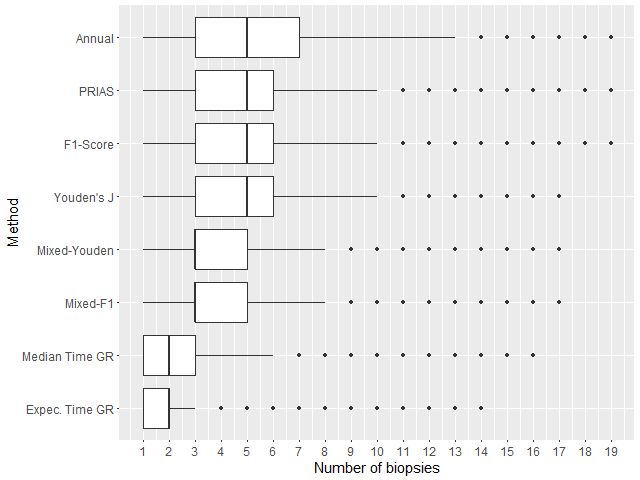
\includegraphics[width=\textwidth]{images/sim_study/nbBoxPlot_all.png}
        \caption{Boxplot for number of biopsies.}
        \label{fig : nbBoxPlot}
    \end{subfigure}
    \begin{subfigure}[b]{0.45\textwidth}
        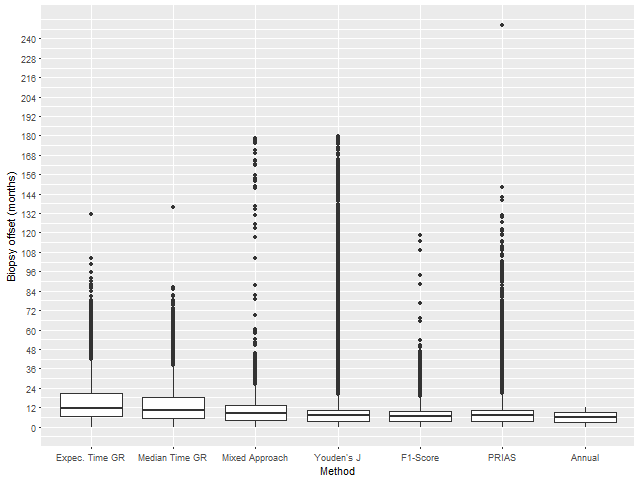
\includegraphics[width=\textwidth]{images/sim_study/offsetBoxPlot_all.png}
        \caption{Boxplot for offset (months)}
        \label{fig : offsetBoxPlot}
    \end{subfigure}      
    \caption{Boxplot for number of biopsies and offset (months), for all of the 63386 patients in the 254 simulated datasets. Method names are abbreviated for ease of graphing.}
\end{figure}
